\begin{center}
{{\Large \sc High-Performance Computing}}
\end{center}
\rule{\textwidth}{1pt}
\begin{description}
\item[Student name and id:] Marie Mørk \{s112770\} Anja Liljedahl Christensen\{s162876\}
 Andreas Vedel Jantzen \{s162858\}
 Anders Launer Bæk \{s160159\}
\item[Team name:] matmult\_MAAA
\item[Hand-in:] OpenMP - Poisson Problem
\end{description}
\rule{\textwidth}{1pt}

\section{Summary}
In this project, the Possion problem is solved numerically using two different methods; Jacobi and Gauss-Seidel. Initially, the methods are implemented in sequential code. This showed that the Gauss-Seidel method needed less iterations for the solution to converge, but at the same time that the Jacobi method was executed faster, due to a higher number of flops/s. The Jacobi method was then parallelized in different versions to investigate the scaling behaviour of the algorithms. Parallelizing not only the algorithm but also the initialization of the matrices resulted in the overall best performance. Different ways of implementing parallelization in the Gauss-Seidel method are explained but not implemented. 

\section{Statement of the problem}
The goal of the project is to determine the steady state heat distribution in a square room with constant heat capacity, a source (radiator), and constant boundary conditions at the walls by solving the Poisson problem numerically. Two different methods are considered for solving the problem; the Jacobi method and the Gauss-Seidel method. Furthermore, the performance of the Jacobi method is to be improved by parallelizing the program using OpenMP. The scaling behaviour of the different versions of the parallelized Jacobi will be compared with that of the Mandelbrot problem. The Gauss-Seidel method cannot be parallelized in the same way as the Jacobi method, but different ways of implementing parallelization using this method will be explained and discussed.\\
% In short, the problem is divided into 4 sub-problems:
% \begin{itemize}
%     \item Sequential Jacobi method
%     \item Sequential Gauss-Seidel method
%     \item OpenMP Jacobi
%     \item OpenMP Gauss-Seidel
% \end{itemize}


\section{Hardware and software}
Specifications of the test environment are listed below:
\begin{itemize}
\item CPU information
\begin{itemize}
\item Vendor ID:             GenuineIntel
\item CPU family:            6
\item Model:                 79
\item Model name:            Intel(R) Xeon(R) CPU E5-2650 v4 @ 2.20GHz
\item CPU MHz:               1297.656
\item L1 (d / i) cache:             32K
\item L2 cache:              256K
\item L3 cache:              30720K
\end{itemize}
\item Compiler settings%\textcolor{red}{and Matrix implementations}
\begin{itemize}
\item The SunCC compiler have been applied with and without compiler optimization using the compiler flags \texttt{-fast -xopenmp} and \texttt{-xopenmp=noopt} respectively. See uploaded \texttt{makefile} for further information.
\end{itemize}
\item Highlights from the batch script. See \texttt{master\_sh.sh} for further information.
\begin{itemize}
\item \texttt{\#BSUB -R "rusage[mem=2048MB] span[hosts=1]"} and \texttt{\#BSUB -n 24} which dedicate the whole host.
\item \texttt{export OMP\_WAIT\_POLICY=active}
\end{itemize}
\end{itemize}


\section{Theory}
The Poisson problem is given by eq. \ref{eq:Poisson}. The goal is to estimate the heat distribution of a room with a radiator.
\begin{equation}
    -f(x,y)
   = \frac{\partial^2 u}{\partial x^2}
      + \frac{\partial^2 u}{\partial y^2}, \qquad (x,y) \in \Omega
\label{eq:Poisson}
\end{equation}
The heat distribution will be estimated using two methods: The Jacobi method given in eq. \ref{eq:jac} and the Gauss-Seidel method given in eq. \ref{eq:gauss}.

\begin{equation}
u_{i,j}^{k+1} = \frac{1}{4} (u_{i-1,j}^{k} +
u_{i+1,j}^{k} + u_{i,j-1}^{k} + u_{i,j+1}^{k} + \Delta^2 f(i,j))
\label{eq:jac}
\end{equation}

\begin{equation}
u_{i,j}^{k+1} = \frac{1}{4} (u_{i-1,j}^{k+1} +
u_{i+1,j}^{k} + u_{i,j-1}^{k+1} + u_{i,j+1}^{k} + \Delta^2 f(i,j))
\label{eq:gauss}
\end{equation}

The main difference between eq. \ref{eq:jac} and eq. \ref{eq:gauss} is that the Gauss-Seidel method uses two updated elements in the update of the center element. The Jacobi method only uses the values from the previous iteration, which makes this method simple to parallelize. \\ 

One of the most important measures of scalability is Amdahl's law. 
It defines the ideal speed-up $S(P)$ for an increase in number of threads when running a given algorithm. Amdahl's law is defined as:
\begin{equation}
    S(P) = \frac{T(1)}{T(P)} = \frac{1}{f/P+1-f}.
    \label{eq:SPp}
\end{equation}

where $S(P)$ is the speed-up as a function of the number of threads $P$. $T(\bullet )$ is the execution time for the given number of threads and $f$ the parallel fraction of the program. 

Equation \ref{eq:SPmax} determines the limit of the theoretical speed-up for a given $f$.
\begin{equation}
S_{max}(f) = \frac{1}{1-f}
\label{eq:SPmax}
\end{equation}

It is possible to achieve a parallel fraction close to $1$ in the Poisson problem, hence the expectation is that a parallel implementation should scale perfectly. 
In reality though, there are numerous things to consider in order to ensure that the program scales properly. 
Amdahl's law neglects the cost of communication, bookkeeping, synchronization, initializing, closing threads etc. The costs influence the properties of the scaling, recall the plot on slide 29 in \texttt{intro\_para2018\_ho.pdf}, found on Inside.

There are other approaches to increase the speed-up in parallel applications executed on multiple sockets. One approach is to initialize the matrices in parallel which "places" matrix elements efficiently according to the assigned threads.
The native \texttt{numactl} command can be used to control the policies for the processes and shared memory. This approach has not been implemented in the project but could be considered as future work. This could speed-up the computation even more. \texttt{NUMA} is a memory placement policy that specifies on what and how many threads the computation has to be processed on.

The number of floating point operations per second (flops/s) is used as a measure of performance when comparing the different implementations. The total number of flops needed to solve the Poisson problem is calculated as the product of the iteration in each of the nested loops times the number of floating point operations performed in the innermost loop. 
This is multiplied by the number of iterations needed in order for the solution to converge (or the maximum number of iterations).
The total number of floating point operations is divided by the time needed to execute the code. The equation becomes:

\begin{equation}
flops/s =  \frac{I \cdot N^2 \cdot O}{T}
\label{eq:flops_time}
\end{equation}
where $I$ is the number of iterations, $N$ is the dimension of the grid (excluding the boarders), $O=10$ is the number of floating point operations in the innermost loop and $T$ the execution time.


\section{Algorithms}
This section introduces the main algorithms used to solve the Poisson problem. Additional algorithms can be found in the appendix. 


\subsection{Sequential code - Jacobi method}
The first function is a sequential implementation of the Jacobi method, see algorithm \ref{alg:jac}. The first input is the problem size, $N$, excluding the borders of the grid. Other inputs are the grid spacing, $\Delta$, the threshold of the convergence, the maximum number of iterations as well as the matrices $f$, $u$ and $u_{old}$. In the implementation, the approximation of $u$ at iteration number $k$ is saved in the matrix $u$. As the calculation of $u$ at timestep $k$ is dependent on the approximation of $u$ at time step $k-1$, the pointers are swapped between $u$ and $u_{old}$ just before the calculations at each iteration commence.


\lstinputlisting[label={alg:jac},caption={Algo. \texttt{jac\_seq\_con()}.},style=CStyle, linerange={28-52-}]{code_2/func.c}

\subsection{Sequential code - Gauss-Seidel method}
The sequential implementation of the Gauss-Seidel method takes the same inputs as the Jacobi method except for $u_{old}$, which is not needed. The code is listed in algorithm \ref{alg:gauss}. 


\lstinputlisting[label={alg:gauss},caption={Algo. \texttt{gauss\_con()}.},style=CStyle, linerange={228-246}]{code_2/func.c}



\subsection{OpenMP Jacobi}
A simple OpenMP version of the Jacobi function is implemented in algorithm \ref{alg:jac_pm}. In this version, the parallel region is set to be around the two inner loops, which loops over the index of the matrices. It is implemented such that the variables $f$, $u$, $u_{old}$, $N$, threads and $d$ are shared, while $i$ and $j$ are private. Each time the innermost loop is reaches, an addition is made to $d$. This results in dataracing, because all threads needs to make an addition to the same shared variable. \\ 
In the second version can be seen in the appendix as algorithm \ref{alg:app_jac_mp_v23}. The difference between the first and second version is that the parallel region has been moved such that it covers the whole while loop. This is an advantage, because the team of parallel threads are created once in the function instead of using fork and join for each iteration. In order to ensure that the threads does not work on different iterations, $k$, at the same time, $k$ is set to be firstprivate. This means that each of the threads gets the same value of k and only one thread updates it in the end of the loop. In the second version, the dataracing of version 1 has been avoided by adding the command \texttt{\#pragma omp for reduction (+ : d)} before the loops over the matrix indices. \\
In the third version, the function in itself is not changed. Instead, the main file is altered such that matrix initializations are parallelized. 


\lstinputlisting[label={alg:jac_pm},caption={Algo. \texttt{jac\_mp()}.},style=CStyle, linerange={54-89}]{code_2/func.c}




The performance of the OpenMP Jacobi is to be compared with the scaling of the Mandelbrot problem. An implementation of the Mandelbrot problem has been given in the week exercise, see algorithm  \ref{alg:app_mandel} in the appendix. \\

\subsection{OpenMP Gauss-Seidel}

The Gauss-Seidel method (eq. \ref{eq:gauss}) is more difficult to parallelize than the Jacobi method.
It is because of the tightly bound nature (the method is coupled to itself by recursion) of the algorithm. Due to this, an OpenMP Gauss-Seidel is not implemented as a part of this project. Instead, different ways of implementing parallelization in Gauss-Seidel will be discussed in this section.\\

The article \citetitle{C2} by \citeauthor{C2} proposes several methods for solving fully coupled systems.
The \textbf{Row Parallel Algorithm} is a brute force parallelization of the Gauss-Seidel method. It takes the inner loop and calculates every row by itself and combines them in the end. 
The \textbf{Column Parallel Algorithm} works in a similar way as the \textbf{Row Parallel Algorithm}, only that it is then the columns that are considered one at a time. Both of these methods reduces the number of syncronizations to be perfromed to $N$ in the case of an $N \times N$ matrix \cite{C2}.

The \textbf{Block-Column Parallel Algorithm} is based on the CUDA library. CUDA only works within thread blocks, hence the system matrix will be divided into $g$ submatrices (or subproblems) each with its own constraints. 
The subproblems can be computed in parallel because the calculations are bounded by its own constraints. 
For every subproblem, the matrix is divided into two blocks; one covering the diagonal of the full original matrix and another with the off-diagonal elements. Every subgroup computes the block with the diagonal elements first and then the off-diagonal. A barrier is introduced in between the calculation of diagonal and off-diagonal blocks.
The subgroups only need $2g$ synchronizations which reduces the dependence of global synchronizations that restricts scalability of the algorithm \cite{C2}.

The \textbf{Atomic Update Counter Parallel Algorithm} does, contrary to the above mentioned, get rid of global synchronization. 
This method stores a shared integer which counts the number of diagonal blocks computed. 
The counter and the revision of the Gauss-Seidel method is presented in the article. Specific hardware is also part of the \textbf{Atomic Update Counter Parallel Algorithm}, because it has to produce an automated-updated counter at the same time as allocating enough memory. This eliminates all synchronizations of the Gauss-Seidel methods \cite{C2}. \\ 

The following methods are derived from the original sequential Gauss-Seidel method from the article \citetitle{C3} by \citeauthor{C3}, \cite{C3}. 
The \textbf{Computation Synchronization} method recalculates the values of $u_{i,j}$ at random.  
The \textbf{Computation Deadlock} method restricts the access to the grid nodes and is hereby forced to parallelize which decreases the computation time.
The \textbf{Interdeterminacy Elimination} method makes the storing of results and current iterations in independent matrices.
The \textbf{Computation Load Balancing} method is as the name suggests a method for balancing the computation load among the used processors. The computation time of the program will hereby depend on the thread with the longest computation time \cite{C3}. 

\newpage

\section{Results}
In the following sections, performance and scaling results from the implemented functions are presented. The functions are tested for different problem sizes and number of threads and optimal choices discussed.

\subsection{Sequential code - Jacobi and Gauss-Seidel method}
First off, the Poisson problem is solved using sequential code and two different methods; Jacobi and Gauss-Seidel. Both programs are tested using matrix sizes $N = 128$ and $N = 256$ and are set to run until they converge. The threshold of the convergence is set to $d = 10 ^{-10}$. In figure \ref{fig:test} the function estimates of $u(x,y)$ based on both methods are shown as heat maps. The estimates obtained are visually similar. 

\begin{figure}[!th]
\centering
\begin{subfigure}{.5\textwidth}
  \centering
  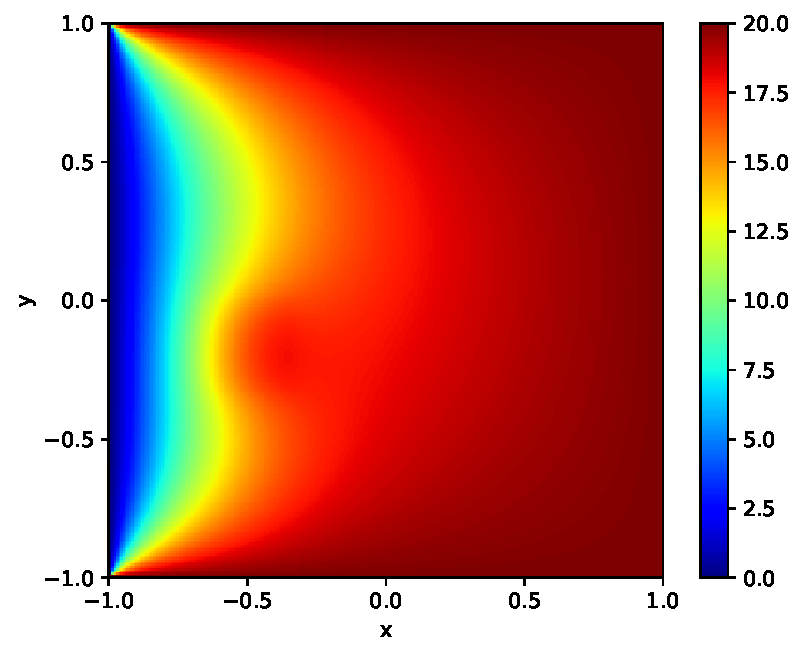
\includegraphics[width=.9\linewidth]{data_2/plots/gaus_con.pdf}
  \caption{Gauss-Seidel}
  \label{fig:}
\end{subfigure}%
\begin{subfigure}{.5\textwidth}
  \centering
  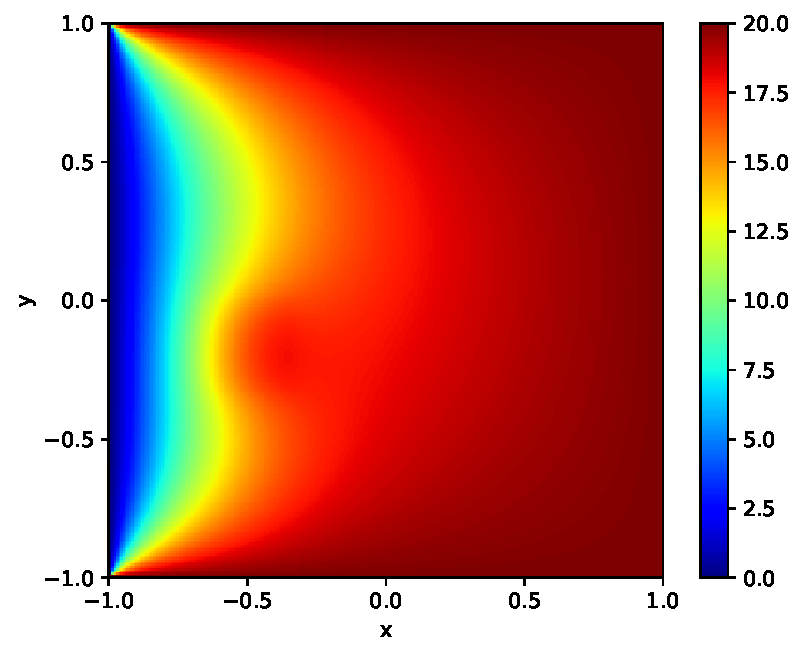
\includegraphics[width=.9\linewidth]{data_2/plots/jac_con.pdf}
  \caption{Jacobi}
  \label{fig:}
\end{subfigure}
\caption{Estimate of the function $u(x,y)$. The problem size of the illustrated heats are $N=256$. See table \ref{tab:seq_par} for further evaluation details.}
\label{fig:test}
\end{figure}

In table \ref{tab:seq_par}, details of the iterations of the two functions for problem sizes $N = 128$ and $256$ are shown. As expected, the memory usage in the Gauss-Seidel method is 2/3 of the Jacobi. This is due to the fact that three matrices are used in the Jacobi method, namely \texttt{f, u} and \texttt{u\_old}, whereas only \texttt{f} and \texttt{u} are needed in Gauss-Seidel. The number of iterations shows how many iterations are needed in order for $u(x,y)$ to converge. For both problem sizes, the Jacobi method needs almost twice as many iterations to reach convergence. In spite of this, the execution time is much larger in the case of Gauss-Seidel because the iterations are coupled, why the compiler optimizer fails to reduce runtime. This also means that fewer iterations and \texttt{mflops} are performed pr. second, as seen in the table. All together this information shows that if parallelization and smart memory allocation is implemented, there is a possibility of a larger performance gain for Gauss-Seidel than for Jacobi. On the other hand, Jacobi is easier parallelized as a result of the uncoupled iterations. 

\begin{table}[!th]
\centering
\begin{tabular}{ll|rrrrr}
&& Memory & Iterations & Duration & Iterations/s & mflops/s \\ \hline
\multirow{2}{*}{128}&\texttt{gauss\_con()}&262144&51225&4.79&10704&1754\\
&\texttt{jac\_seq\_con()}&393216&101831&1.76&57717&9456\\\hline
\multirow{2}{*}{256}&\texttt{gauss\_con()}&1048580&194176&73.38&2646&1734\\
&\texttt{jac\_seq\_con()}&1572860&390976&25.80&15153&9931\\
\end{tabular}
\caption{Comparison of the Jacobi method and Gauss-Seidel method.}
\label{tab:seq_par}
\end{table}

\subsection{OpenMP Jacobi}

The Jacobi method can be parallelized and run on multiple cores with shared memory using OpenMP. In the optimal setting the speed-up of increasing the number of cores is 1, i.e. using 2 cores instead of 1 should make the program run twice as fast. As discussed in the theory section OpenMP has several constructs which can be used to optimize the parallelization and ensure correctness. In the following sections, parallelized versions of the Jacobi method are implemented and continuously improved. For this purpose the number of iterations are fixed such that $k$ runs from 1 to \texttt{max\_iter} (with \texttt{max\_iter} = 5000) in order to best compare the efficiency of the different parallelized versions. Each version is run on 1, 4, 8, 16, and 24 threads for 4 different problem sizes $N \in \{256, 512, 1024, 2048\}$.

The first simple version will be used as a baseline.

\subsubsection{Version 1}

The first simple version has 2 parallel constructsm see algorithm \ref{alg:jac}: The first one contains a single-construct to make one of the threads extract the number of threads running the program. The second is nested within the while loop and contains a loop-construct such that the iterations from the outer for-loop (i.e. the rows) are distributed among the threads.

Figure \ref{fig:jac_comp_measure_v1} shows how increasing the number of threads for different problem sizes increases the number of flops per second. The gain is especially evident for $N = 512$ and $N = 1024$, while for $N = 2048$ there is no efficiency improvement when increasing the number of threads beyond $8$. This is explained by the fact that when $N$ is this size the problem does not fit within the 3 caches, hence
memory has to be fetched from the RAM which is significantly slower and hereby slows down the process.

In figure \ref{fig:scaling_mp_jac_v1} the speed-up for each problem size is compared to the theoretical speed-up. For problem sizes $256$, $512$, and $1024$ there is a clear correlation between problem size and speed-up, i.e. as the problem size increases so does the speed-up. This, however, is not the case for $N=2048$ which is as before most likely linked to the amount of needed memory. Since there are two sockets each running $12$ threads, they are forced to communicate when the number of threads exceeds 12 which could potentially slow down the process when the problem is large enough. 


\begin{figure}[H]
\centering
\begin{tikzpicture}[scale = 0.85]
\begin{axis}[
width=17cm, height=8cm,     % size of the image
grid = major,
grid style={dashed, gray!30},
xmode=log,log basis x=10,
ymin=0,    % start the diagram at this 
ymax=155000, % end   the diagram at this 
axis background/.style={fill=white},
ylabel=Mflops/s,
xlabel=Memory/kbytes,
legend pos=north east]
\addplot[mark=*, green] table [x=mem, y=mflops, col sep=comma]{data_2/plots/program_jac_mp_ncore_1.txt};
\addlegendentry{1 thread}
\addplot[mark=*, orange] table [x=mem, y=mflops, col sep=comma]{data_2/plots/program_jac_mp_ncore_4.txt};
\addlegendentry{4 threads}
\addplot[mark=*, blue] table [x=mem, y=mflops, col sep=comma]{data_2/plots/program_jac_mp_ncore_8.txt};
\addlegendentry{8 threads}
\addplot[mark=*, red] table [x=mem, y=mflops, col sep=comma]{data_2/plots/program_jac_mp_ncore_16.txt};
\addlegendentry{16 threads}
\addplot[mark=*, black] table [x=mem, y=mflops, col sep=comma]{data_2/plots/program_jac_mp_ncore_24.txt};
\addlegendentry{24 threads}
\end{axis}
\end{tikzpicture}
\caption{Jacobi version 1.}
\label{fig:jac_comp_measure_v1}
\end{figure}

\begin{figure}[H]
\centering
\begin{tikzpicture}[scale = 0.85]
\begin{axis}[
width=9cm, height=9cm,
grid = major,
grid style={dashed, gray!30},
xmin=0,
ymin=0,
ymax=24,
xmax=24,% end   the diagram at this 
/pgfplots/xtick={0,2,...,24},
/pgfplots/ytick={0,2,...,24},
axis background/.style={fill=white},
ylabel=S(P),
xlabel=P,
legend pos=north west]
\addplot[green, domain=0:25, no markers,samples=100] {x};
\addlegendentry{Theo.}
\addplot[mark=*, orange] table [x=ncore, y=SP, col sep=comma]{data_2/plots/program_jac_mp_SP_256.txt};
\addlegendentry{256}
\addplot[mark=*, blue] table [x=ncore, y=SP, col sep=comma]{data_2/plots/program_jac_mp_SP_512.txt};
\addlegendentry{512}
\addplot[mark=*, red] table [x=ncore, y=SP, col sep=comma]{data_2/plots/program_jac_mp_SP_1024.txt};
\addlegendentry{1024}
\addplot[mark=*, black] table [x=ncore, y=SP, col sep=comma]{data_2/plots/program_jac_mp_SP_2048.txt};
\addlegendentry{2048}
\end{axis} 
\end{tikzpicture}
\caption{Scaling Jacobi version 1.}
\label{fig:scaling_mp_jac_v1}
\end{figure}




\subsubsection{Version 2}

For version 2 the second parallel construct is moved out to include the while-loop as well, seen in algorithm \ref{alg:app_jac_mp_v23}. In the previous version the master thread distributed the iterations among the threads each time the while-loop counter $k$ was incremented by 1. Hence, there was a fork and a join of the threads for each $k$ from 1 to \texttt{max\_iter} which resulted in a lot of waiting time in between the actual computations. In this version the iterations are only distributed among the threads once which should decrease the waiting time. Now the pointers have to be swapped in parallel but this should only be done by one of the threads to avoid data racing. Therefore it is also crucial that the threads use the same iteration $k$ by declaring the variable as a \texttt{firstprivate}.

Figure \ref{fig:jac_comp_measure_v2} shows how the performance is now increased for each combination of problem size and number of threads (apart from 1 thread). The improvement is the most evident when using 24 threads, while it seems there is no improvement when using 1 thread. This makes sense since there is nothing running in parallel when using only 1 thread.

In figure \ref{fig:scaling_mp_jac_v2} it is hard to detect any improvement for problem sizes 256, 512, and 1024, while the speed-up for $N = 2048$ is a little better beyond 12 threads.

\begin{figure}[H]
\centering
\begin{tikzpicture}[scale = 0.85]
\begin{axis}[
width=17cm, height=8cm,     % size of the image
grid = major,
grid style={dashed, gray!30},
xmode=log,log basis x=10,
ymin=0,    % start the diagram at this 
ymax=155000, % end   the diagram at this 
axis background/.style={fill=white},
ylabel=Mflops/s,
xlabel=Memory/kbytes,
legend pos=north east]
\addplot[mark=*, green] table [x=mem, y=mflops, col sep=comma]{data_2/plots/program_jac_mp_v2_ncore_1.txt};
\addlegendentry{1 thread}
\addplot[mark=*, orange] table [x=mem, y=mflops, col sep=comma]{data_2/plots/program_jac_mp_v2_ncore_4.txt};
\addlegendentry{4 threads}
\addplot[mark=*, blue] table [x=mem, y=mflops, col sep=comma]{data_2/plots/program_jac_mp_v2_ncore_8.txt};
\addlegendentry{8 threads}
\addplot[mark=*, red] table [x=mem, y=mflops, col sep=comma]{data_2/plots/program_jac_mp_v2_ncore_16.txt};
\addlegendentry{16 threads}
\addplot[mark=*, black] table [x=mem, y=mflops, col sep=comma]{data_2/plots/program_jac_mp_v2_ncore_24.txt};
\addlegendentry{24 threads}
\end{axis} 
\end{tikzpicture}
\caption{Jacobi version 2.}
\label{fig:jac_comp_measure_v2}
\end{figure}


\begin{figure}[H]
\centering
\begin{tikzpicture}[scale = 0.85]
\begin{axis}[
width=9cm, height=9cm,
grid = major,
grid style={dashed, gray!30},
xmin=0,
ymin=0,
ymax=24,
xmax=24,% end   the diagram at this 
/pgfplots/xtick={0,2,...,24},
/pgfplots/ytick={0,2,...,24},
axis background/.style={fill=white},
ylabel=S(P),
xlabel=P,
legend pos=north west]
\addplot[green, domain=0:25, no markers,samples=100] {x};
\addlegendentry{Theo.}
\addplot[mark=*, orange] table [x=ncore, y=SP, col sep=comma]{data_2/plots/program_jac_mp_v2_SP_256.txt};
\addlegendentry{256}
\addplot[mark=*, blue] table [x=ncore, y=SP, col sep=comma]{data_2/plots/program_jac_mp_v2_SP_512.txt};
\addlegendentry{512}
\addplot[mark=*, red] table [x=ncore, y=SP, col sep=comma]{data_2/plots/program_jac_mp_v2_SP_1024.txt};
\addlegendentry{1025}
\addplot[mark=*, black] table [x=ncore, y=SP, col sep=comma]{data_2/plots/program_jac_mp_v2_SP_2048.txt};
\addlegendentry{2048}
\end{axis} 
\end{tikzpicture}
\caption{Scaling Jacobi version 2.}
\label{fig:scaling_mp_jac_v2}
\end{figure}




\subsubsection{Version 3}

For the final version the Jacobi method itself is the same as version 2, but this time the initialization of the matrices is also parallelized. Hence, the data is pre-distributed among the threads to make it more accessible when running the actual program. 

In figure \ref{fig:jac_comp_measure_v3} it is once again obvious that the larger of the problem sizes are the ones to exploit the further parallelization the most. Especially $N = 2048$ utilizes the parallelized initialization of the matrices, which makes sense given the large memory consumption.

By considering figure \ref{fig:scaling_mp_jac_v3} it is clear that the problem sizes $256$ and $512$ experience the best improvement of speed-up, while $N=1024$ seems to be unchanged.

\begin{figure}[H]
\centering
\begin{tikzpicture}[scale = 0.85]
\begin{axis}[
width=17cm, height=8cm,     % size of the image
grid = major,
grid style={dashed, gray!30},
xmode=log,log basis x=10,
ymin=0,    % start the diagram at this 
ymax=155000, % end   the diagram at this 
axis background/.style={fill=white},
ylabel=Mflops/s,
xlabel=Memory/kbytes,
legend pos=north east]
\addplot[mark=*, green] table [x=mem, y=mflops, col sep=comma]{data_2/plots/program_jac_mp_v3_ncore_1.txt};
\addlegendentry{1 thread}
\addplot[mark=*, orange] table [x=mem, y=mflops, col sep=comma]{data_2/plots/program_jac_mp_v3_ncore_4.txt};
\addlegendentry{4 threads}
\addplot[mark=*, blue] table [x=mem, y=mflops, col sep=comma]{data_2/plots/program_jac_mp_v3_ncore_8.txt};
\addlegendentry{8 threads}
\addplot[mark=*, red] table [x=mem, y=mflops, col sep=comma]{data_2/plots/program_jac_mp_v3_ncore_16.txt};
\addlegendentry{16 threads}
\addplot[mark=*, black] table [x=mem, y=mflops, col sep=comma]{data_2/plots/program_jac_mp_v3_ncore_24.txt};
\addlegendentry{24 threads}
\end{axis} 
\end{tikzpicture}
\caption{Jacobi version 3.}
\label{fig:jac_comp_measure_v3}
\end{figure}



\begin{figure}[H]
\centering
\begin{tikzpicture}[scale = 0.85]
\begin{axis}[
width=9cm, height=9cm,
grid = major,
grid style={dashed, gray!30},
xmin=0,
ymin=0,
ymax=24,
xmax=24,% end   the diagram at this 
/pgfplots/xtick={0,2,...,24},
/pgfplots/ytick={0,2,...,24},
axis background/.style={fill=white},
ylabel=S(P),
xlabel=P,
legend pos=north west]
\addplot[green, domain=0:25, no markers,samples=100] {x};
\addlegendentry{Theo.}
\addplot[mark=*, orange] table [x=ncore, y=SP, col sep=comma]{data_2/plots/program_jac_mp_v3_SP_256.txt};
\addlegendentry{256}
\addplot[mark=*, blue] table [x=ncore, y=SP, col sep=comma]{data_2/plots/program_jac_mp_v3_SP_512.txt};
\addlegendentry{512}
\addplot[mark=*, red] table [x=ncore, y=SP, col sep=comma]{data_2/plots/program_jac_mp_v3_SP_1024.txt};
\addlegendentry{1024}
\addplot[mark=*, black] table [x=ncore, y=SP, col sep=comma]{data_2/plots/program_jac_mp_v3_SP_2048.txt};
\addlegendentry{2048}
\end{axis} 
\end{tikzpicture}
\caption{Scaling Jacobi version 3.}
\label{fig:scaling_mp_jac_v3}
\end{figure}

%DET ER YDERST fedt at se 2048 hvor P er 1,2 og 4





\subsubsection{Comparison}

In figure \ref{fig:jac_comp_measure_v123} the efficiency of the 3 different OpenMP Jacobi methods are compared for 4 different problem sizes (the same as before) using 8 and 16 cores. Version 1 is outperformed by version 2 and 3 using both 8 and 16 threads. With 8 threads version 2 and 3 are practically indistinguishable, while using 16 threads the best performing version alternates between 2 and 3 depending on the problem size.

\begin{figure}[H]
\centering
\begin{tikzpicture}[scale = 1]
\begin{axis}[
width=17cm, height=8cm,     % size of the image
grid = major,
grid style={dashed, gray!30},
xmode=log,log basis x=10,
ymin=0,    % start the diagram at this 
ymax=155000, % end   the diagram at this 
axis background/.style={fill=white},
ylabel=Mflops/s,
xlabel=Memory/kbytes,
legend pos=north east]
\addplot[mark=*, purple] table [x=mem, y=mflops, col sep=comma]{data_2/plots/program_jac_mp_ncore_8.txt};
\addlegendentry{v1\_8}
\addplot[mark=*, orange] table [x=mem, y=mflops, col sep=comma]{data_2/plots/program_jac_mp_v2_ncore_8.txt};
\addlegendentry{v2\_8}
\addplot[mark=*, green] table [x=mem, y=mflops, col sep=comma]{data_2/plots/program_jac_mp_v3_ncore_8.txt};
\addlegendentry{v3\_8}


\addplot[mark=*, red] table [x=mem, y=mflops, col sep=comma]{data_2/plots/program_jac_mp_ncore_16.txt};
\addlegendentry{v1\_16}
\addplot[mark=*, black] table [x=mem, y=mflops, col sep=comma]{data_2/plots/program_jac_mp_v2_ncore_16.txt};
\addlegendentry{v2\_16}
\addplot[mark=*, blue] table [x=mem, y=mflops, col sep=comma]{data_2/plots/program_jac_mp_v3_ncore_16.txt};
\addlegendentry{v3\_16}

\end{axis}
\end{tikzpicture}
\caption{Jacobi version 1, 2 and 3 for 8 and 16 threads.}
\label{fig:jac_comp_measure_v123}
\end{figure}

\subsection{Mandelbrot}

The scaling behaviour of the Jacobi method and of the Mandelbrot algorithm is given in figure \ref{fig:scaling_comp_opt} and in figure \ref{fig:scaling_non_comp_opt} with and without compiler optimization flags repectively.

The four methods have been evaluated for $N=1024$ and with $ max_{iter} = 5000$.

\begin{figure}[H]
\begin{subfigure}{.5\textwidth}
\centering
\begin{tikzpicture}[scale = 1]
\begin{axis}[
width=8cm, height=8cm,
grid = major,
grid style={dashed, gray!30},
xmin=0,
ymin=0,
ymax=24,
xmax=24,% end   the diagram at this 
/pgfplots/xtick={0,2,...,24},
/pgfplots/ytick={0,2,...,24},
axis background/.style={fill=white},
ylabel=S(P),
xlabel=P,
legend pos=north west]
\addplot[green, domain=0:25, no markers,samples=100] {x};
\addlegendentry{Theo.}
\addplot[mark=*, black] table [x=ncore, y=SP, col sep=comma]{data_2/plots/program_mandel.txt};
\addlegendentry{Mandel}
\addplot[mark=*, red] table [x=ncore, y=SP, col sep=comma]{data_2/plots/program_jac_mp_SP.txt};
\addlegendentry{Jacobi\_v1}
\addplot[mark=*, blue] table [x=ncore, y=SP, col sep=comma]{data_2/plots/program_jac_mp_v2_SP.txt};
\addlegendentry{Jacobi\_v2}
\addplot[mark=*, orange] table [x=ncore, y=SP, col sep=comma]{data_2/plots/program_jac_mp_v3_SP.txt};
\addlegendentry{Jacobi\_v3}
\end{axis} 
\end{tikzpicture}
\caption{Optimized}
\label{fig:scaling_comp_opt}
\end{subfigure}%
\begin{subfigure}{.5\textwidth}
\centering
\begin{tikzpicture}[scale = 1]
\begin{axis}[
width=8cm, height=8cm,
grid = major,
grid style={dashed, gray!30},
xmin=0,
ymin=0,
ymax=24,
xmax=24,% end   the diagram at this 
/pgfplots/xtick={0,2,...,24},
/pgfplots/ytick={0,2,...,24},
axis background/.style={fill=white},
ylabel=S(P),
xlabel=P,
legend pos=north west]
\addplot[green, domain=0:25, no markers,samples=100] {x};
\addlegendentry{Theo.}
\addplot[mark=*, black] table [x=ncore, y=SP, col sep=comma]{data_2/plots/program_mandel_non.txt};
\addlegendentry{Mandel\_non}
\addplot[mark=*, red] table [x=ncore, y=SP, col sep=comma]{data_2/plots/program_jac_mp_SP_non.txt};
\addlegendentry{Jacobi\_v1\_non}
\addplot[mark=*, blue] table [x=ncore, y=SP, col sep=comma]{data_2/plots/program_jac_mp_v2_SP_non.txt};
\addlegendentry{Jacobi\_v2\_non}
\addplot[mark=*, orange] table [x=ncore, y=SP, col sep=comma]{data_2/plots/program_jac_mp_v3_SP_non.txt};
\addlegendentry{Jacobi\_v3\_non}
\end{axis} 
\end{tikzpicture}
\caption{Non optimized}
\label{fig:scaling_non_comp_opt}
\end{subfigure}
\caption{The plots shows the scaling as function of number of threads P with following compiler flags: \texttt{-fast -xopenmp} and \texttt{-xopenmp=noopt} for \ref{fig:scaling_comp_opt} and \ref{fig:scaling_non_comp_opt} respectively.}
%\label{fig:test}
\end{figure}

There is a slight difference between the three versions of the Jacobi method when not using the mentioned compiler optimization flags, see figure \ref{fig:scaling_non_comp_opt}. The three versions follows each other for a given $P$ except for $P=24$.

It can be concluded that the current implementation of the Mandelbrot algorithm (algo. \ref{alg:app_mandel}) does not scale as the implementations of the Jacobi method, see table \ref{tab:avergae_f} where $f$ have been derived from eq. \ref{eq:SPp}.
An explanation for the scaling of the Mandelbrot is the unbalanced work load in the while loop for the assigned threads. A solution to this could be dynamic scheduling of the work balance.

Table \ref{tab:avergae_f} reports the average values of $f$ for the curves in figure \ref{fig:scaling_comp_opt} and figure \ref{fig:scaling_non_comp_opt}. $f$ have been derived from eq. \ref{eq:SPp}.

\begin{table}[H]
\centering
\begin{tabular}{l|cc}
Algo. & $f_{opt}$ & $f_{non}$  \\\hline
\texttt{manddel()} & 0.730 & 0.726\\
\texttt{jac\_mp()} & 0.976 & 0.972\\
\texttt{jac\_mp\_v2()} & 0.974 & 0.974\\
\texttt{jac\_mp\_v3()} & 0.976 & 0.980\\
\end{tabular}
\caption{Average value of $f$ for each algorithm. The values in the second column corresponds to figure \ref{fig:scaling_comp_opt} and the third column corresponds to figure \ref{fig:scaling_non_comp_opt}. }
\label{tab:avergae_f}
\end{table}
The max speed-up limit for \texttt{jac\_mp\_v3()} is $S_{max}(0.976)=\left\lfloor  41 \right\rfloor$. The max speed-up limit for \texttt{mandel()} is $S_{max}(0.730)=\left\lfloor  3\right\rfloor$, see eq. \ref{eq:SPmax}.


\section{Conclusion}
The sequential codes for the Jacobi and Gauss-Seidel methods showed that while the Gauss-Seidel method needs less iterations for the solution to converge, it is still much slower than Jacobi. This is because more floating point operations are performed pr. second in Jacobi. From the analysis of the performance of the sequential programs it was found that parallelization and smarter data allocation could enhance the performance of both methods, but that the possible gain might be higher for using Gauss-Seidel, due to convergence being reached after fewer iterations and the fact that this method uses less memory. 


As previously discussed the parallelized third version of the Jacobi method clearly improved the efficiency (number of flops per second) compared to the first and second version. The improvement of the speed-up is not that evident for the problem sizes 256, 512, and 1024, but when the problem doesn't fit within the first three caches and has to be stored in the RAM, there is some gain in speed-up when optimizing the parallelization – both with respect to the Jacobi method itself and the initialization of the matrices.

For future work it could be beneficial to implement the \texttt{NUMA} control policy.
